\section{真实硬件实验与结果评估}
\label{sec:4}

前文交代了 WFB-FL 怎样在原始无线帧路径上组织收发协同与调度。进入物理实验，我们关注两件事。一是这六项无线参数在真实硬件上能支持到什么范围，二是在学习任务、节点规模与计算条件保持一致时，不同的无线配置怎样改变多客户端训练的通信表现与整轮耗时。为此，我们在由真实边缘计算节点与消费级 802.11 无线网卡搭建的物理测试台上开展实验评估。

\subsection{实验设置}

真实硬件实验平台由 1 台参数服务端与 10 台边缘客户端组成，节点计算设备采用 Jetson Orin Nano 边缘计算板卡，各节点均外接消费级 RTL8812AU 双频 USB 无线网卡，驱动采用开源的 rtl88xxau\_wfb 实现。全部节点部署于面积约 120 平方米的典型室内办公环境中，各客户端分散放置在不同工位与隔断间，节点间距在 3 至 12 米之间，包含直射视距与穿透隔断的非视距反射路径，构成典型的室内多径与阴影衰落效应。无线信道处于包含邻近商用 Wi-Fi 弱干扰的真实室内电磁环境。在联邦学习工作负载方面，实验采用 ResNet-18 深度神经网络模型与 CIFAR-10 图像分类数据集构建同步联邦学习任务，单次模型广播分发的数据文件大小固定为 40 MiB（约 41.9 MB）。整个实验过程基于真实物理硬件、真实操作系统网络栈与真实无线链路收发闭环运行，不采用网络仿真器或单机多进程模拟。

\subsection{可配置无线参数}

在此硬件平台上，WFB-FL 支持对工作信道、信道带宽、调制编码方案（MCS）、保护间隔（GI）、前向纠错（FEC）冗余以及发射功率六项关键无线参数实施显式配置。六项参数平级列出，各自对应物理层收发与链路控制层不同的调控维度，共同为构建不同的无线工作条件提供参数依据。Table~\ref{tab:2} 汇总了当前硬件环境下各项无线参数的可配置取值与硬件支持范围。

% 原稿标记保留：**[Table 2 占位 六项无线参数的可配置取值与硬件支持范围]**

% 原稿题注保留：> Table 2 平级列出信道、带宽、MCS、保护间隔、前向纠错和发射功率的可配置取值与硬件支持范围，为三种无线配置提供依据。

\begin{table*}[tb]
\caption{六项无线参数的可配置取值与硬件支持范围。}
\label{tab:2}
\centering
\small
\renewcommand{\arraystretch}{1.25}
\setlength{\tabcolsep}{5pt}
\begin{tabularx}{\textwidth}{@{}>{\raggedright\arraybackslash}p{0.15\textwidth}YY@{}}
\toprule
\textbf{无线参数类别} & \textbf{典型可配置取值范围} & \textbf{硬件与系统支持范围及约束} \\
\midrule
\textbf{工作信道} & 2.4 GHz（Ch 1 至 13）与 5 GHz 频段主流信道（如 5 GHz Ch 157） & 取决于 RTL8812AU 射频芯片支持范围及所在地区无线电管理频谱法规 \\
\textbf{信道带宽} & 20 MHz 与 40 MHz（HT20 / HT40+） & 取决于网卡射频基带芯片与驱动对频宽切换的支持能力 \\
\textbf{调制编码（MCS）} & MCS 0 至 MCS 7（802.11n 单天线单流调制编码，BPSK 至 64-QAM） & 取决于射频基带支持的调制阶数与编码率 \\
\textbf{保护间隔（GI）} & 长保护间隔（Long GI, 800 ns）与短保护间隔（Short GI, 400 ns） & 取决于基带芯片符号时序控制与驱动对短保护间隔特性的支持 \\
\textbf{前向纠错（FEC）} & Cauchy-Reed-Solomon 纠错码冗余（RS(8, 10) 至 RS(8, 14) 块级冗余配置） & 由链路控制层软件实现，受边缘节点 CPU 编解码计算负载约束 \\
\textbf{发射功率} & 10 dBm 至 20 dBm（综合实验固定为 17 dBm） & 受 RTL8812AU 射频功放物理上限及 Linux 内核无线驱动接口支持范围约束 \\
\bottomrule
\end{tabularx}
\end{table*}

\subsection{完整 FL 综合实验}

为评估物理无线条件对联邦学习端到端训练的影响，我们设计并执行了多客户端联邦学习综合实验。该实验回答一个核心问题。当模型架构、训练数据集、参与节点规模、本地计算步数、工作信道（固定为 5 GHz Ch 157）、发射功率（固定为 17 dBm）以及空间物理拓扑保持一致时，不同的预设无线配置怎样改变多客户端联邦学习的通信表现与整体轮次耗时。

依据 Table~\ref{tab:2} 所列的硬件支持范围，实验预设了三种典型无线配置，分别命名为稳健性优先、折中以及吞吐优先。配置命名仅代表预先设定的参数设计取向，具体参数组合在正式实验数据采集前固定，三组配置全部无偏地进入端到端综合实验，不根据后验测试表现对配置进行反向筛选。稳健性优先配置采用 20 MHz 信道带宽、MCS 2（QPSK 3/4）、长保护间隔与 RS(8, 14) 纠错冗余（约 42.8\% 冗余），旨在恶劣信道下优先保证低误码与确定性；折中配置采用 20 MHz 信道带宽、MCS 4（16-QAM 3/4）、短保护间隔与 RS(8, 12) 纠错冗余（33.3\% 冗余），在基础速率与抗扰度间寻求平衡；吞吐优先配置采用 40 MHz 信道带宽、MCS 6（64-QAM 3/4）、短保护间隔与 RS(8, 10) 纠错冗余（20.0\% 冗余），旨在最大化瞬时物理发射速率。

在综合实验执行与统计口径上，每种配置均独立执行 10 次完整的多客户端联邦学习训练，每次训练包含 5 轮严格闭环训练，同一次训练中的各轮次仅反映训练时序推进，不作为独立重复样本。综合实验对全部尝试的完成情况进行完整记录与如实呈现，不静默删除任何失败或超时的运行。核心评价指标包括模型下行有效吞吐、客户端更新提交情况与完整轮次耗时三项。模型下行有效吞吐定义为单次广播的模型文件总大小除以全体目标客户端均成功完成完整模型文件接收与校验所需的总交付时间；客户端更新提交情况记录各客户端在限时发送窗口轮转调度下的轮内实际提交时刻与提交成功状态；完整轮次耗时严格从服务端发布该轮模型开始计时，历经下行可靠广播、各客户端本地计算以及多客户端轮转上行提交，直至服务端收齐本轮预期有效更新并完成算法聚合时为止。客户端在本地校验模型后即可立即训练（单节点单轮计算耗时约 10 至 12 秒），部分较快完成计算的客户端会在其他客户端仍在计算时提前提交更新，下行交付、本地训练与上行回传在时间上形成流水线重叠，各阶段耗时不能简单相加。

% 原稿标记保留：**[Figure 4 占位 综合实验结果组合图]**

% 原稿题注保留：> Figure 4 展示三种预设无线配置下的模型下行有效吞吐、客户端更新提交情况和完整轮次耗时，交代全部尝试的完成情况。

\begin{figure*}[tb]
\centering
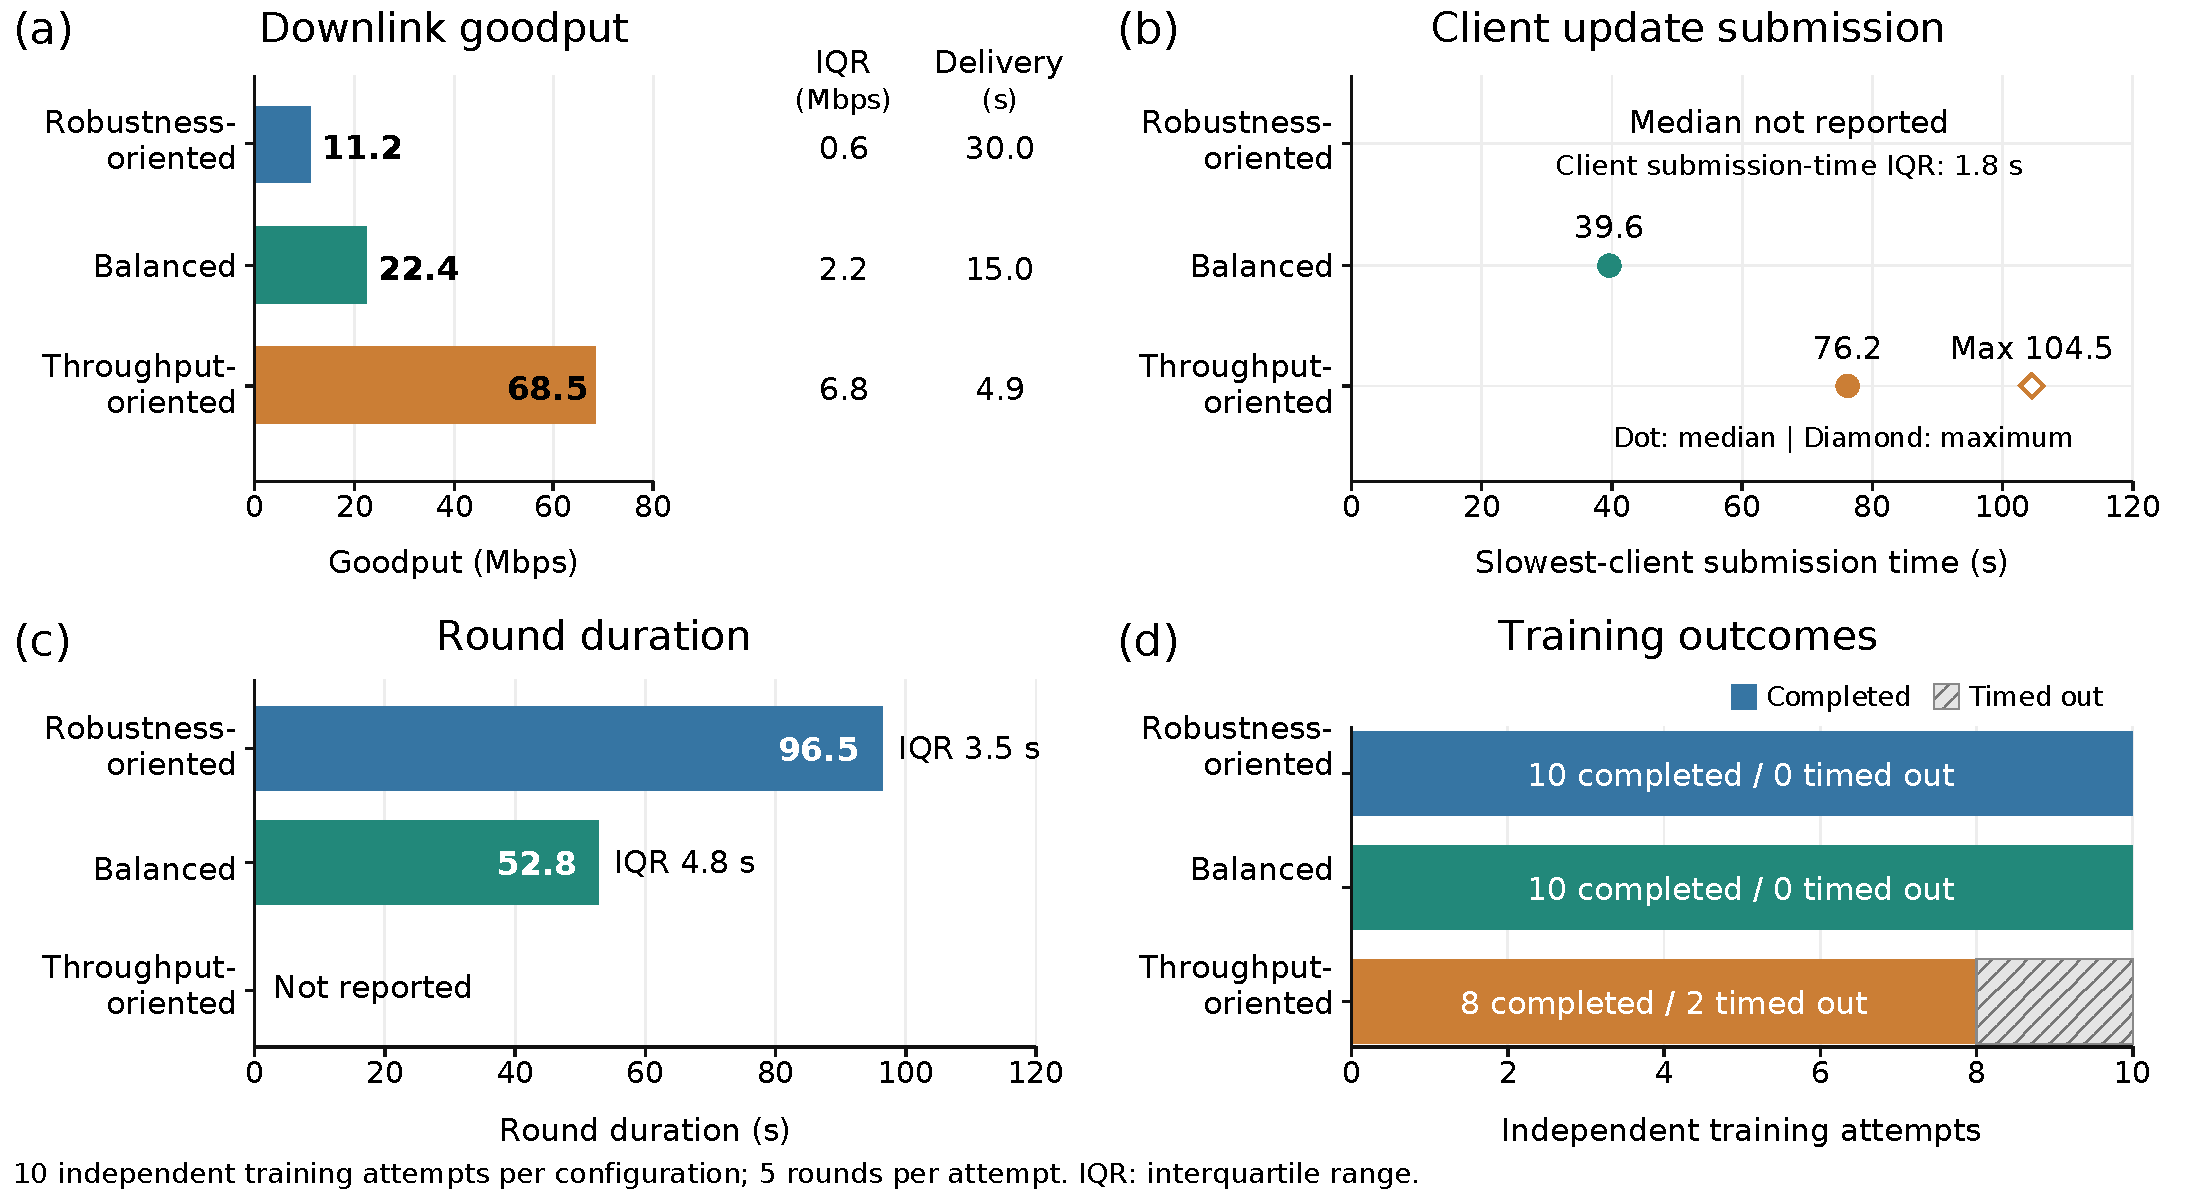
\includegraphics[width=\textwidth]{figure4.pdf}
\caption{三种预设无线配置的综合实验结果：（a）下行有效吞吐；（b）客户端更新提交；（c）完整轮次耗时；（d）训练尝试的完成情况。每种配置独立尝试 10 次训练，每次 5 轮；IQR 表示四分位距。}
\label{fig:4}
\end{figure*}

Figure~\ref{fig:4} 综合展示了三种预设无线配置在多次独立训练中的测量结果分布。定量比较表明，不同的无线参数组合对联邦学习端到端轮次呈现出显著不同的系统影响。在模型下行分发阶段，吞吐优先配置依托高阶调制与较高带宽，下行有效吞吐达到 68.5 Mbps（四分位距 6.8 Mbps），交付耗时仅为 4.9 秒；但在上行更新阶段，高阶调制在实际空间多径扰动下容易丢包，导致部分弱信号客户端在轮转调度中经历更多重传，最慢客户端的提交耗时呈现严重长尾拖尾，中位数达到 76.2 秒（极值达 104.5 秒）；相比之下，稳健性优先配置在下行阶段的有效吞吐为 11.2 Mbps（四分位距 0.6 Mbps），分发耗时为 30.0 秒，但各客户端提交时刻表现出高度集中的一致性（四分位距仅 1.8 秒，无长尾拖尾），整轮耗时分布在中位数 96.5 秒（四分位距 3.5 秒）；折中配置的下行有效吞吐达到 22.4 Mbps（四分位距 2.2 Mbps，分发耗时 15.0 秒），各客户端提交平稳推进（最慢客户端耗时中位数 39.6 秒），整轮耗时中位数为 52.8 秒（四分位距 4.8 秒）。在全部 10 次独立训练尝试中，稳健性优先配置成功闭环 10 次（10 次成功，0 次超时），折中配置成功闭环 10 次（10 次成功，0 次超时），吞吐优先配置成功闭环 8 次，其余 2 次因隔断弱信号节点上行停滞超时未完成（8 次成功，2 次超时失败）。

上述测量结果表明，在相同的算法与计算负载下，底层物理无线条件直接改变模型分发与更新提交的时间分配，名义物理速率最高并不保证整轮训练耗时最短。这一系统含义进一步印证了将无线链路转变为显式可控实验对象的必要性。同时，本实验的证据边界严格立足于固定拓扑、特定硬件与上述预设配置组合的整体表现，结果差异归因于整套无线配置在特定物理环境中的综合效果，不孤立归因于某一单项物理参数，不将配置映射为外部设备类型，亦不据此声称该组合在算法收敛精度上带来改善或优于商用黑盒 Wi-Fi 协议栈。
